\section{Direktumrichter (AC--AC-Umrichter ohne Zwischenkreis)}

Ein Direktumrichter wandelt eine dreiphasige Wechselspannung mit Frequenz $f_1$
\textbf{direkt} in eine Wechselspannung mit veränderlicher Frequenz $f_2$ und Amplitude,
\textbf{ohne Verwendung eines Gleichstrom-Zwischenkreises}.

Im Gegensatz zu Wechselrichtern erfolgt die Energiewandlung in \textbf{einem einzigen Schaltprozess}:
\[
\text{AC}_{f_1} \;\longrightarrow\; \text{AC}_{f_2}
\]

Typische Anwendungen:
\begin{itemize}
\item Niederdrehzahl-Grossantriebe,
\item Walzwerke,
\item Schiffantriebe,
\item Mühlen- und Ofenantriebe.
\end{itemize}

\subsection{Grundprinzip der direkten AC--AC-Wandlung}

% --- bestehende Grafik ---
\begin{center}
    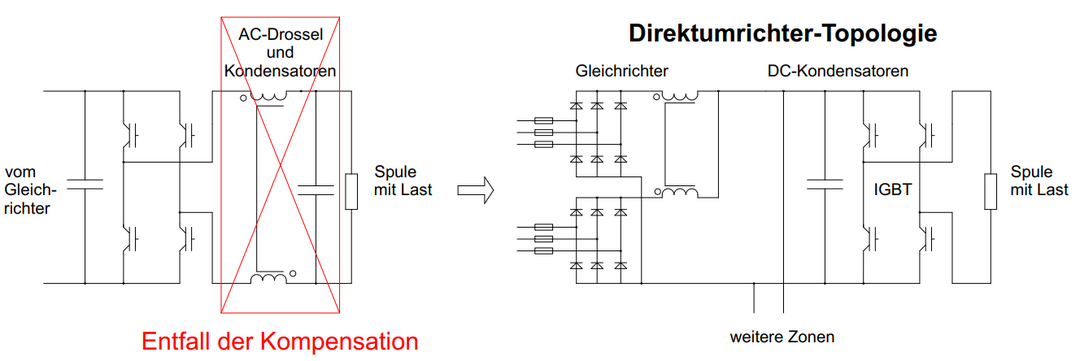
\includegraphics[width=0.85\linewidth]{images/direktumrichtergrund.png}
\end{center}

Der Direktumrichter verbindet jede Eingangsphase direkt mit jeder Ausgangsphase
über bidirektionale Schalter.

Mathematisch wird die Ausgangsspannung als zeitvariante Linearkombination
der Eingangsspannungen gebildet:

\[
\boxed{
\begin{bmatrix}
u_a(t)\\
u_b(t)\\
u_c(t)
\end{bmatrix}
=
\mathbf{M}(t)
\begin{bmatrix}
u_{R}(t)\\
u_{S}(t)\\
u_{T}(t)
\end{bmatrix}
}
\]

mit:

\begin{itemize}
    \item $u_{R},u_{S},u_{T}$: Eingangsphasenspannungen (Netz),
    \item $u_a,u_b,u_c$: Ausgangsphasenspannungen (Last),
    \item $\mathbf{M}(t)$: zeitabhängige Schaltmatrix mit Einträgen $m_{ij}(t) \in \{0,1\}$.
\end{itemize}

Jeder Matrixeintrag beschreibt:
\[
m_{ij}(t) =
\begin{cases}
1, & \text{Phase } j \text{ ist mit Ausgang } i \text{ verbunden} \\
0, & \text{sonst}
\end{cases}
\]

\crd{\textrightarrow\ Der Direktumrichter realisiert eine zeitvariable Abbildung zwischen Eingangs- und Ausgangsphasen.}

---

\subsection{Schaltungsstruktur (Matrixumrichter)}

% --- bestehende Grafik ---
\begin{center}
    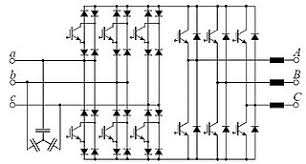
\includegraphics[width=0.85\linewidth]{images/direktumrichter_matrix.png}
\end{center}

Ein dreiphasiger Direktumrichter besitzt:

\[
\boxed{3 \times 3 = 9 \text{ bidirektionale Schalter}}
\]

Jeder Schalter muss:

\begin{itemize}
\item Strom in beide Richtungen leiten können,
\item Spannung in beide Richtungen sperren können,
\item kurzschluss- und unterbrechungsfrei schalten.
\end{itemize}

Typische Realisierung:
\[
\text{Bidirektionaler Schalter} = \text{2 antiparallele IGBTs mit Dioden}
\]

---

\subsection{Bildung der Ausgangsfrequenz}

Die Ausgangsspannung wird durch zeitliche Gewichtung der Eingangsphasen gebildet.

Idealisierte Darstellung für eine Ausgangsphase:

\[
\boxed{
u_a(t) = \alpha_R(t) u_R(t) + \alpha_S(t) u_S(t) + \alpha_T(t) u_T(t)
}
\]

mit:

\begin{itemize}
    \item $\alpha_R(t),\alpha_S(t),\alpha_T(t)$: zeitabhängige Schaltfunktionen,
    \item $\alpha_R+\alpha_S+\alpha_T = 1$ (keine Unterbrechung der Last).
\end{itemize}

Die Grundfrequenz der Ausgangsspannung ist:

\[
\boxed{f_2 = f_{\text{ref}}}
\]

wobei das Referenzsignal aus der Modulation erzeugt wird.

---

\subsection{Frequenzgrenze des Direktumrichters}

Die Ausgangsfrequenz ist durch die Kommutierung begrenzt:

\[
\boxed{f_2 < \frac{1}{2} f_1}
\]

Begründung:

\begin{itemize}
\item Jede Ausgangshalbwelle benötigt mehrere sichere Netzkommutierungen.
\item Die Netzspannung muss die Stromumlenkung erzwingen.
\item Bei zu hoher $f_2$ ist keine sichere Kommutierung mehr möglich.
\end{itemize}

Typischer Praxisbereich:
\[
f_2 \le 0.3 \, f_1
\]

---

\subsection{Leistungsfluss und Vierquadrantenbetrieb}

Momentanleistung:
\[
\boxed{p(t) = u_2(t)\, i_2(t)}
\]

Mittlere Leistung:
\[
\boxed{P = \frac{1}{T} \int_0^T u_2(t)\, i_2(t)\, dt}
\]

Da keine Diodenstrecken vorhanden sind, gilt:

\begin{itemize}
\item Strom kann Vorzeichen wechseln,
\item Spannung kann Vorzeichen wechseln,
\item Energie kann in beide Richtungen fliessen.
\end{itemize}

Damit ist möglich:

\[
\boxed{
(u,i) \in \{(+,+), (+,-), (-,+), (-,-)\}
}
\]

\crd{\textrightarrow\ Direktumrichter sind grundsätzlich vierquadrantenfähig.}

---

\subsection{Kommutierung als zentrales Problem}

% --- bestehende Grafik ---
\begin{center}
    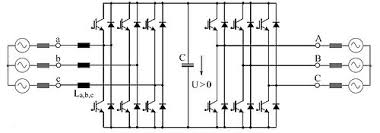
\includegraphics[width=0.85\linewidth]{images/direktumrichter_kommutierung.png}
\end{center}

Während der Kommutierung gilt zwingend:

\[
\boxed{
\begin{aligned}
&\text{Kein Kurzschluss zweier Netzphasen},\\
&\text{Kein Unterbrechen des Laststroms}.
\end{aligned}
}
\]

Formale Nebenbedingungen:

\[
\sum_{j \in \{R,S,T\}} m_{ij}(t) = 1 
\quad \forall i \in \{a,b,c\}
\]

und:

\[
\sum_{i \in \{a,b,c\}} m_{ij}(t) \le 1 
\quad \forall j \in \{R,S,T\}
\]

Bedeutung:

\begin{itemize}
\item Jede Lastphase ist immer mit genau einer Netzphase verbunden.
\item Keine zwei Lastphasen dürfen gleichzeitig dieselbe Netzphase kurzschliessen.
\end{itemize}

\crd{\textrightarrow\ Die Kommutierungslogik bestimmt die Komplexität des Direktumrichters.}

---

\subsection{Ausgangsströme bei R--L-Last}

Für jede Ausgangsphase gilt:

\[
\boxed{
u_k(t) = R i_k(t) + L \frac{di_k(t)}{dt},
\qquad k \in \{a,b,c\}
}
\]

Zeitkonstante:
\[
\boxed{\tau = \frac{L}{R}}
\]

Allgemeine Lösung bei konstantem $u_k$:

\[
\boxed{
i_k(t) = \frac{u_k}{R} + \left(i_k(t_0) - \frac{u_k}{R}\right) e^{-(t-t_0)/\tau}
}
\]

---

\subsection{Eigenschaften und Einordnung}

\begin{itemize}
    \item Sehr robuster Industrieumrichter.
    \item Hoher Wirkungsgrad (keine Zwischenkreisverluste).
    \item Begrenzter Frequenzbereich.
    \item Sehr komplexe Kommutierungssteuerung.
\end{itemize}

---

\subsection{Vergleich Direktumrichter -- Zwischenkreis-Wechselrichter}

\begin{center}
\begin{tabular}{l|c|c}
 & Direktumrichter & Wechselrichter \\ \hline
Zwischenkreis & nein & \cbl{ja} \\
Energiepuffer & keiner & \cbl{Kondensator} \\
AC--AC-Wandlung & direkt & \cbl{zweistufig} \\
Frequenzbereich & $f_2 < 0.5 f_1$ & \cbl{frei wählbar} \\
PWM notwendig & nein & \cbl{ja} \\
Kommutierung & netzgeführt & \cbl{selbstgeführt} \\
\end{tabular}
\end{center}

---

\subsection{Merksätze (Prüfungskern)}

\begin{itemize}
    \item Direktumrichter: direkte AC--AC-Wandlung ohne Zwischenkreis.
    \item Ausgangsspannung ist Linearkombination der Eingangsspannungen.
    \item Ausgangsfrequenz ist grundsätzlich begrenzt.
    \item Kommutierung ist das zentrale technische Problem.
    \item Vierquadrantenbetrieb ist ohne Zusatzschaltung möglich.
\end{itemize}
